\documentclass[aspectratio=169,10pt]{beamer}
\usetheme{Madrid}
\usecolortheme{dolphin}
\usepackage{amsmath,booktabs}
\title{Fair Allocation of Job Training under Uncertain Treatment Benefits}
\subtitle{ICT 5143 AFGML Capstone — Problem 6}
\author{Akshay Wali \and Mohit Das}
\institute{261090830018 \quad $\vert$ \quad 261090840018}
\date{}

\begin{document}
\begin{frame}
\titlepage
\end{frame}

\begin{frame}{The decision problem}
\begin{itemize}
\item A public programme has limited job-training places.
\item Ranking people by predicted post-training earnings is not the same as ranking by additional benefit from training.
\item Estimated benefits are uncertain, especially in small demographic groups.
\end{itemize}
\vspace{0.4em}
\[
\tau(x,a)=E[Y(1)-Y(0)\mid X=x,A=a]
\]
\centering
\textbf{Question:} Can uncertainty-aware allocation improve the worst-group benefit without sacrificing too much total value?
\end{frame}

\begin{frame}{Data, causal model and estimation}
\begin{columns}[T]
\column{0.47\textwidth}
\textbf{Experimental NSW subset}
\begin{itemize}
\item 445 participants
\item 185 treated; 260 controls
\item Outcome: real 1978 earnings
\item Recorded race $\times$ age groups
\item Male-only: no gender fairness claim
\end{itemize}
\column{0.53\textwidth}
\textbf{Causal workflow}
\begin{enumerate}
\item Causal DAG and back-door reasoning
\item Difference-in-means
\item Outcome regression
\item IPW
\item Cross-fitted AIPW
\item Honest train/validation/test policy evaluation
\end{enumerate}
\end{columns}
\end{frame}

\begin{frame}{Policies and fairness}
\begin{itemize}
\item Baselines: random, predicted earnings, CATE ranking, shallow tree and equal-rate allocation.
\item Comparators: point-estimate group-benefit constraint and group-benefit LCB constraint.
\item Capacities: 20\%, 40\%, 60\%.
\end{itemize}
\[
V(\pi)=E[\pi(X)\{Y(1)-Y(0)\}]
\]
\[
B_g(\pi)=E[\pi(X)\{Y(1)-Y(0)\}\mid G=g]
\]
\textbf{Primary fairness target:} minimum supported-group incremental benefit. Allocation-rate gap is a separate access diagnostic.
\end{frame}

\begin{frame}{Feasibility and held-out value at 40\% capacity}
\centering
\begin{tabular}{lrrr}
\toprule
Rule & Original folds & Fold refits & Held-out value\\
\midrule
Unconstrained & 5/5 & 500/500 & 1,074.67\\
Point-estimate floor & 2/5 & 158/500 & Unavailable\\
LCB floor & \alert{0/5} & \alert{0/500} & \alert{Unavailable}\\
\bottomrule
\end{tabular}

\vspace{1em}
\begin{block}{Lower-confidence-bound rule}
The rule selected no feasible policy in the original outer folds. Its full-sample held-out value was unavailable. Refitting held the validation and test participants fixed.
\end{block}
\end{frame}

\begin{frame}{NSW policy results}
\centering
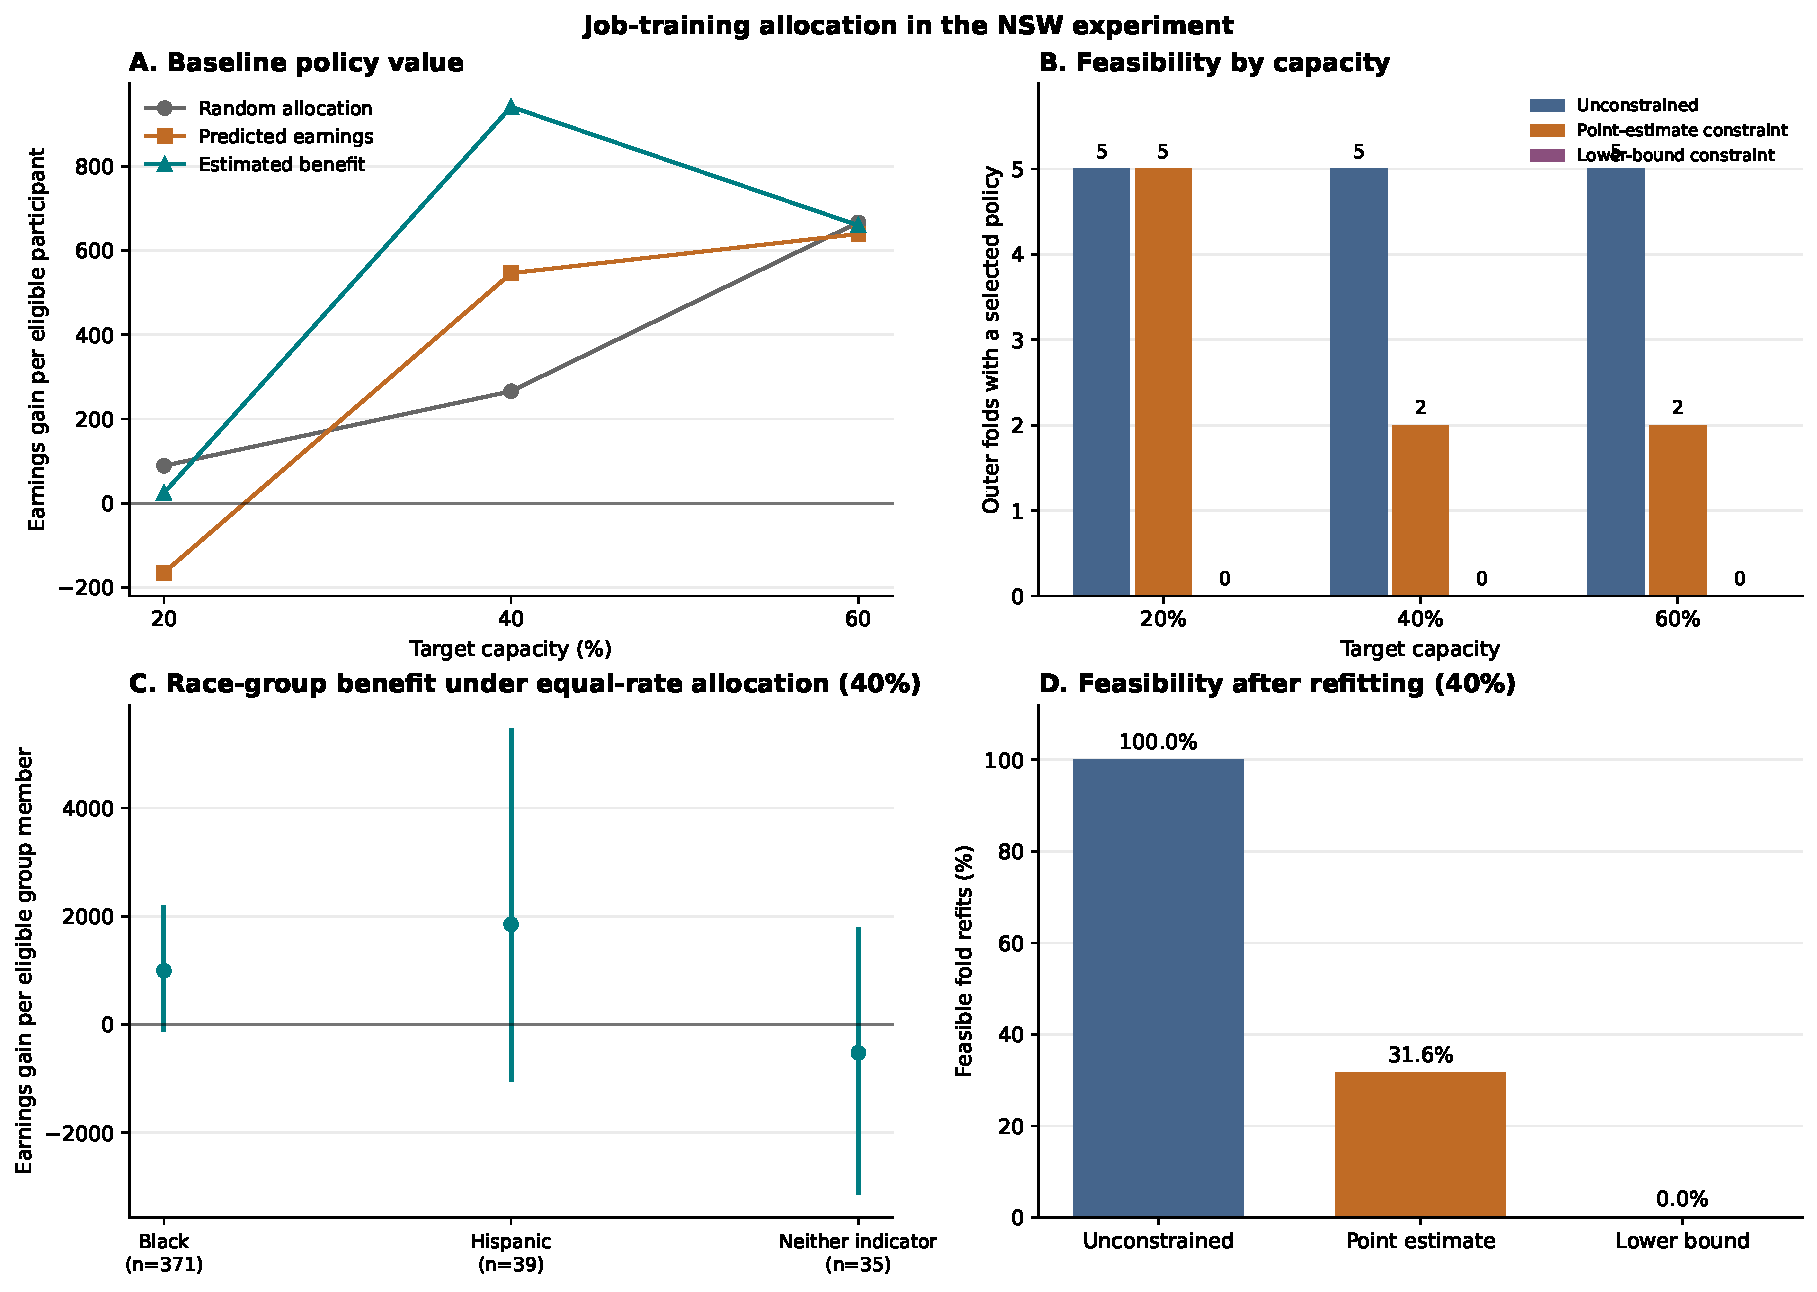
\includegraphics[width=\linewidth,height=0.64\textheight,keepaspectratio]{results/figures/nsw_main_results.pdf}

\small Panels B and D show feasibility. Zero bars indicate zero feasible selections. At 40\% capacity the LCB held-out value was unavailable.
\end{frame}

\begin{frame}{Ablations and reproducibility}
\begin{itemize}
\item Replacing the LCB with a point estimate increased feasible original folds from 0 to 2 out of 5.
\item Removing the benefit floor increased feasible original folds to 5 out of 5.
\item Benefit ranking exceeded earnings ranking by an estimated 394.98 per eligible participant. The paired 95\% interval was [$-110.36$, 856.59].
\item The full pipeline completed in a fresh environment. Four CSVs matched exactly by SHA-256.
\end{itemize}
\end{frame}
\end{document}
